\section{Design and Implementation}

The idea is to add another layer on top of Beer, that based on \color{red} Algorithm \color{black}, will encrypt and decrypt the messages that the different devices will exchange between each other.

\begin{figure}[h]
	\centering
	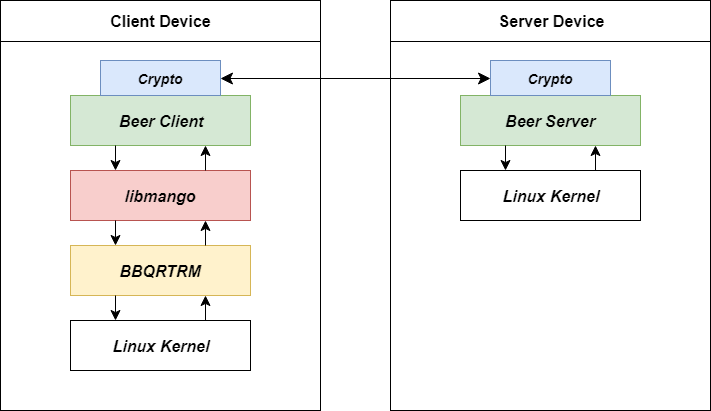
\includegraphics[scale=0.5]{Images/Diagrams/Beer+Crypto_Devices}
	\caption{Beer+Crypto Devices Types}
\end{figure}

First of all when the Client is instantiated it will run the Multi-party Key Agreement in order to calculate the shared key. Next, once it gets in the "ONLINE" state, it will start exchanging data with the other devices.\par
\color{red} Crypto \color{black} is integrated in the Beer Framework and allows the system to encrypt/decrypt messages based on the shared key and the \color{red} Crypto Algorithm.